\documentclass[UTF8,a4paper,10pt,fontset=none]{ctexart}
\usepackage[margin=20mm,headheight=15pt,footskip=12mm]{geometry}
\setCJKmainfont{Noto Serif CJK SC}
\setCJKsansfont{Noto Sans CJK SC}
\setCJKmonofont{Noto Sans Mono CJK SC}
\setmainfont{TeX Gyre Pagella}
\setsansfont{TeX Gyre Heros}
\setmonofont{DejaVu Sans Mono}[Scale=0.82]
\usepackage{amsmath,amssymb,graphicx,booktabs,tabularx,array,longtable,xcolor,fancyhdr,enumitem,listings,xurl,hyperref,lastpage}
\definecolor{brand}{HTML}{176B78}
\definecolor{ink}{HTML}{25333D}
\definecolor{pale}{HTML}{F0F5F6}
\hypersetup{colorlinks=true,linkcolor=brand,urlcolor=brand,pdfauthor={PulsarV},bookmarksnumbered=true}
\graphicspath{{../../images/}}
\ctexset{section={format=\Large\sffamily\bfseries\color{brand}},subsection={format=\large\sffamily\bfseries\color{ink}}}
\pagestyle{fancy}\fancyhf{}
\fancyhead[L]{\small\sffamily MOHISM VINS}
\fancyhead[R]{\small\sffamily\DocName}
\fancyfoot[L]{\small\sffamily\DocCode\enspace |\enspace Rev. 1.0}
\fancyfoot[R]{\small\thepage\ /\pageref*{LastPage}}
\renewcommand{\headrulewidth}{0.3pt}
\setcounter{tocdepth}{1}
\setlength{\parindent}{0pt}\setlength{\parskip}{6pt}
\renewcommand{\arraystretch}{1.38}
\setlist{nosep,leftmargin=1.6em,topsep=4pt}
\newcolumntype{Y}{>{\raggedright\arraybackslash}X}
\newcommand{\code}[1]{\nolinkurl{#1}}
\setlength{\emergencystretch}{2em}
\newcommand{\note}[1]{\par\smallskip\noindent\colorbox{pale}{\parbox{\dimexpr\linewidth-2\fboxsep}{#1}}\par\smallskip}
\lstset{basicstyle=\ttfamily\footnotesize,backgroundcolor=\color{pale},frame=none,breaklines=true,columns=fullflexible,keepspaces=true,showstringspaces=false,xleftmargin=6pt,xrightmargin=6pt,aboveskip=7pt,belowskip=7pt}
\newcommand{\cover}[2]{
\begin{titlepage}
{\sffamily\color{brand}\Large MOHISM\hfill\small TECHNICAL DOCUMENTATION}\par
\vspace{16mm}
{\sffamily\bfseries\fontsize{34}{42}\selectfont MOHISM VINS}\par
\vspace{3mm}{\sffamily\fontsize{24}{32}\selectfont\DocName}\par
\vspace{4mm}{\color{brand}\large 双目视觉惯性设备}\par
\vspace{10mm}
\includegraphics[width=\linewidth]{#1}\par
\vfill
\begin{tabularx}{\linewidth}{@{}lY@{}}\toprule
文档编号 & \DocCode\\
文档版本 & 1.0\quad /\quad 2026-10-30\\
固件基线 & 0.5.0，源码基线 \code{03d9960}\\
作者 & PulsarV\quad\href{mailto:zhijiatao@outlook.com}{zhijiatao@outlook.com}\\
内容 & #2\\\bottomrule
\end{tabularx}
\vspace{6mm}
{\footnotesize 原创硬件与文档采用 CC BY-NC-SA 4.0；软件许可按仓库 \code{LICENSING.md}。}
\end{titlepage}}

\newcommand{\DocName}{使用手册}
\newcommand{\DocCode}{MV-UM-001}
\hypersetup{pdftitle={MOHISM VINS 使用手册}}
\begin{document}
\cover{02_MoSense_USB.png}{连接与识别、图像采集、参数配置、标定、维护及故障排查}
\tableofcontents
\vspace{6mm}
\section*{阅读约定}
本手册以 Linux 笔记本为主机，命令在仓库根目录执行。代码块上方注明“主机”或“板端”；\code{/dev/videoN}、\code{/dev/videoM} 和 \code{/dev/ttyACM0} 为示例，应替换为识别到的设备节点。

首次使用顺序：连接设备 → 识别视频和串口 → 读取参数 → 保存预览图 → 完成标定 → 启用 VIO → 检查状态与里程计。默认 \code{calibrated: 0} 时只提供预览与配置，深度为零，不输出有效里程计。
\note{镜像写卡会覆盖目标存储。操作前核对磁盘型号、容量和挂载点，保留标定、参数和地图备份。}
\newpage
\section{连接设备}
\subsection{准备物品}
准备支持 USB 2.0 High Speed 数据传输的 Type-C 线缆、Linux 笔记本及装有固件的 SD 卡。串口调试可使用 picocom；视频节点查看使用 v4l-utils。早期启动诊断另备电平兼容的 UART 转接器。

保持镜头清洁，避免遮挡视野和散热鳍片。将设备固定后再连接线缆，给插头保留应力释放空间。改变镜头焦点或相机安装关系后重新检查标定。
\begin{center}
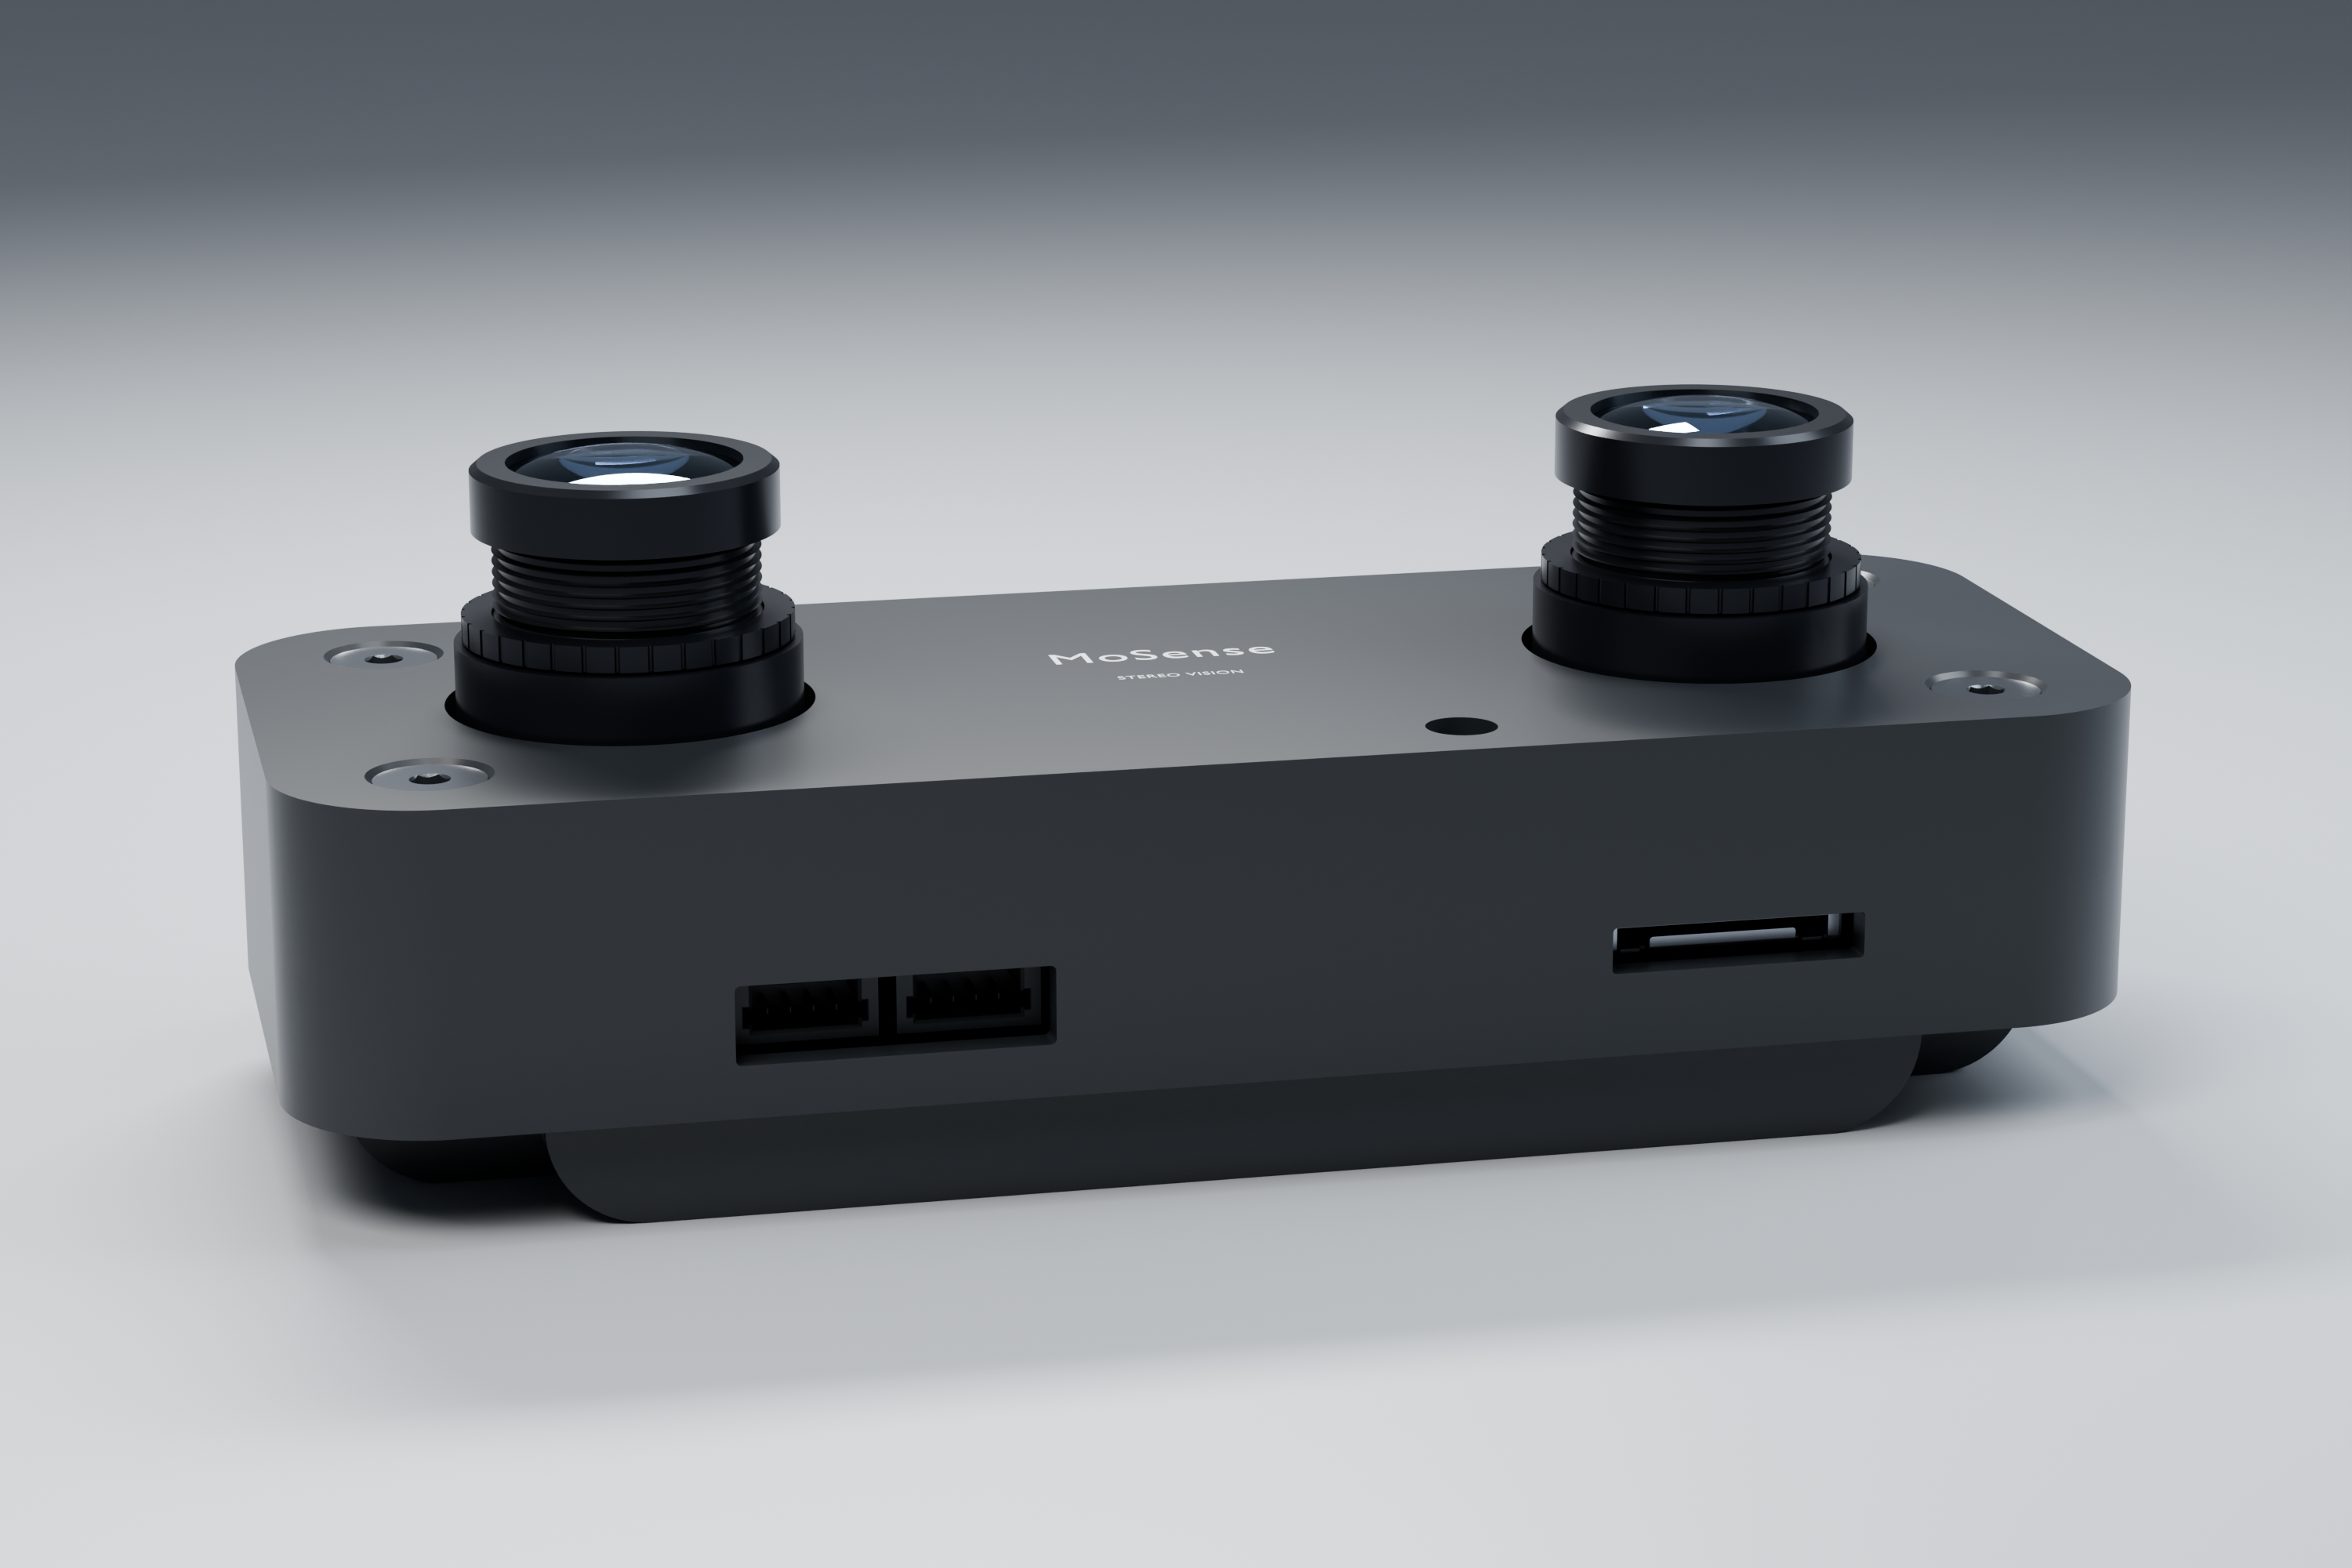
\includegraphics[width=.82\linewidth,height=67mm,keepaspectratio]{04_MoSense_Interfaces.png}\\
{\small 双目、USB、存储与扩展接口的结构视角}
\end{center}

\subsection{主机检查}
连接 USB 后执行：
\begin{lstlisting}
lsusb
lsusb -t
v4l2-ctl --list-devices
ls -l /dev/ttyACM* /dev/video*
\end{lstlisting}
Linux 固件通常显示 \code{1d6b:0104}。在 \code{lsusb -t} 中确认 480M，视频由 uvcvideo 驱动，两个串口由 cdc\_acm 驱动。同一设备包含两个视频功能和两个串口；视频驱动还可能创建元数据节点。

\par\noindent\begin{tabularx}{\linewidth}{@{}p{28mm}Y@{}}\toprule
接口 & 用途\\\midrule
双目 UVC & 640$\times$200 YUYV，左右并排\\
深度 UVC & 320$\times$200 Z16，毫米\\
MAVLink ACM & 参数、状态与里程计，接口 4/5\\
调试 ACM & 系统日志、登录与 Shell，接口 6/7\\\bottomrule
\end{tabularx}\par
\newpage
\section{识别接口与安装主机工具}
\subsection{识别串口角色}
主机执行以下命令，查看 \code{ID_USB_INTERFACE_NUM}：
\begin{lstlisting}
udevadm info -q property -n /dev/ttyACM0
udevadm info -q property -n /dev/ttyACM1
\end{lstlisting}
MAVLink 使用控制接口 04，调试使用 06。设备编号受插拔和其他串口影响，不使用固定编号判断角色。权限不足时，将当前用户加入系统的串口访问组并重新登录；常见组名为 dialout。视频访问组通常为 video。

\subsection{识别视频节点}
\begin{lstlisting}
v4l2-ctl -d /dev/videoN --all
v4l2-ctl -d /dev/videoN --list-formats-ext
v4l2-ctl -d /dev/videoM --list-formats-ext
\end{lstlisting}
选择具备 Video Capture 能力的节点。YUYV 640$\times$200 为双目；Z16 320$\times$200 为深度。Metadata Capture 节点用于元数据，不是普通图像节点。

\subsection{安装 Python 工具}
主机进入仓库执行：
\begin{lstlisting}
python3 -m venv .venv
. .venv/bin/activate
pip install -r host/requirements.txt
\end{lstlisting}
如果发行版未提供 venv，先通过包管理器安装 Python venv 组件。后续命令在已激活虚拟环境的终端中运行。主机图像工具依赖 OpenCV，串口工具使用 MAVLink。

\subsection{读取参数}
\begin{lstlisting}
python host/mohism.py --serial /dev/ttyACM0 params
python host/mohism.py --serial /dev/ttyACM0 odometry
\end{lstlisting}
第一条命令读取参数；第二条持续接收位姿。若没有有效位姿，先查看 \code{VIO_VALID} 与标定状态，再检查初始化、特征数量和 IMU 日志。
\newpage
\section{预览、保存图像与接收位姿}
\subsection{保存双目与深度}
主机执行：
\begin{lstlisting}
python host/mohism.py images --stereo /dev/videoN --depth /dev/videoM --output capture --frames 100
\end{lstlisting}
输出目录包含 \code{stereo/}、\code{depth/} 和到达时间记录。左右灰度图为 8 位 PNG，深度为 16 位 PNG。

双目左右各 320$\times$200，显示时应保留原始灰度。深度单位为毫米，0 表示无效；读取时保留 uint16，不转换成 RGB 或 8 位灰度。双目与深度独立计数，按各自到达记录整理文件。

\subsection{理解深度更新}
深度计算和视频输出分别调度。深度可重复最近一次计算结果；超过 200 ms 无新结果时清零。未标定、关闭估计或无法形成有效深度时也输出零值。统计有效深度率时应区分视频缓冲数量和独立计算结果数量。

\subsection{启用与停用 VIO}
\begin{lstlisting}
python host/mohism.py --serial /dev/ttyACM0 set VIO_ENABLE 0
python host/mohism.py --serial /dev/ttyACM0 set VIO_ENABLE 1
python host/mohism.py --serial /dev/ttyACM0 odometry
\end{lstlisting}
关闭 VIO 后仍保留预览。重新开启后需要初始化与连续视觉更新预热。首次启动建议保持静止约 0.5 秒，机体前向避免接近竖直；运动初始化需要足够的视觉和惯性激励。

\subsection{接收端坐标处理}
输出采用 LOCAL\_FRD / BODY\_FRD，四元数 $[w,x,y,z]$ 表示机体到世界的旋转。位置在世界坐标中，速度在机体坐标中。时间戳为板端单调时钟微秒，不是 UTC。

跟踪恢复、重新启用或地图修正时，\code{reset_counter} 可能递增；接收端按计数变化划分轨迹段。计数为模 256，进程重启归零，同时检查时间戳是否重新开始。协方差和角速度字段为 NaN，quality 为 $-1$。
\newpage
\section{参数与性能设置}
\subsection{MAVLink 参数}
\par\noindent\begin{tabularx}{\linewidth}{@{}p{35mm}p{18mm}Y@{}}\toprule
参数 & 默认 & 用途\\\midrule
\code{VIO_ENABLE} & 1 & 估计启停\\
\code{VIO_VALID} & 0 & 只读，有效状态\\
\code{FW_VERSION} & 500 & 只读，固件 0.5.0\\
\code{SYNC_MAX_MS} & 2 & 左右时间差门限，ms\\
\code{ACC_NOISE} & 0.1 & 加速度白噪声密度\\
\code{GYRO_NOISE} & 0.01 & 角速度白噪声密度\\
\code{ACC_BIAS_RW} & 0.0001 & 加速度偏置随机游走\\
\code{GYRO_BIAS_RW} & 0.00001 & 角速度偏置随机游走\\\bottomrule
\end{tabularx}\par
写入示例：
\begin{lstlisting}
python host/mohism.py --serial /dev/ttyACM0 set ACC_NOISE 0.15
python host/mohism.py --serial /dev/ttyACM0 params
\end{lstlisting}
写入后读取确认。错误类型、NaN、越界或只读参数写入会回传当前值。参数保存在 \code{/userdata/mohism-params.yml}；写盘失败时回滚。噪声参数使用标定结果，修改后在后续图像处理周期生效。

\subsection{帧率配置}
板端 \code{/etc/mohism/performance.conf} 的默认内容：
\begin{lstlisting}
CAPTURE_FPS=120
USB_FPS=60
DEPTH_FPS=30
\end{lstlisting}
采集支持 15/30/60/120，USB 支持 15/30/60；深度请求不超过采集率。深度 USB 频率取 USB 与深度请求的较小值。降低深度计算频率可减少稠密匹配负载。

修改后在板端依次执行：
\begin{lstlisting}
/etc/init.d/S50mohism-vins stop
/etc/init.d/S40mohism-usb restart
/etc/init.d/S50mohism-vins start
\end{lstlisting}
USB 重启会断开调试终端。从 UART 执行上述操作，或将完整命令放入脱离终端运行的脚本；重新识别主机节点后再打开视频流。
\newpage
\section{标定与配置部署}
\subsection{双目标定}
保持 \code{calibrated: 0}，使用尺寸已知的棋盘，采集至少 15 组清晰图像对。改变距离、倾角和棋盘在视野中的位置，覆盖画面边缘。示例命令在主机执行：
\begin{lstlisting}
python host/mohism.py images --stereo /dev/videoN --frames 200 --output chessboard
python host/calibrate_stereo.py chessboard/stereo --columns 9 --rows 6 --square-metres 0.025 --output stereo-measured.yml
\end{lstlisting}
方格边长使用米，内角点行列数与实际棋盘一致。脚本输出重投影 RMS，拒绝大于 1 px 的结果。脚本处理原生 1280$\times$800 与 USB 320$\times$200 的尺度关系。

\subsection{相机与 IMU 联合标定}
联合标定需要原始轴向的加速度、角速度、左右原始图像及同一设备时基下的采集时间戳。普通 \code{arrival.csv} 是主机到达时间记录，不作为采集时间戳输入 Kalibr。Allan 分析使用静止长时 IMU 数据；联合标定使用覆盖各旋转轴和视野的运动数据。

本手册主流程对应 0.5.0 发布接口。专用标定采集工具应与对应固件版本成套使用；输出包需包含原始数据、采样比例、时间戳来源、序号与完整性报告。Kalibr 导出主题可使用 \code{/imu0}、\code{/cam0/image_raw} 与 \code{/cam1/image_raw}。时间校准需处理 IMU IRQ 偏移与图像时间戳相对曝光中心的偏移。

\subsection{配置字段}
\par\noindent\begin{tabularx}{\linewidth}{@{}p{31mm}Y@{}}\toprule
字段 & 含义\\\midrule
\code{K1/K2, D1/D2} & 原生分辨率相机内参与畸变\\
\code{R, T} & $X_{right}=R X_{left}+T$，平移单位米\\
\code{Rbc, tbc} & $X_{body}=R_{bc}X_{left}+t_{bc}$\\
\code{Rbi} & IMU 原始轴到机体 FRD 的旋转\\
\code{imu_offset} & 加到 IMU IRQ 时间的偏移，秒\\
\code{left, right, imu} & 输入设备节点\\
\code{calibrated} & 0 为预览，1 为启用标定\\\bottomrule
\end{tabularx}\par
将标定结果合并到完整 YAML，放入板端 \code{/userdata/calibration.yml}，设置 \code{calibrated: 1} 后执行 \code{/etc/init.d/S50mohism-vins restart}。镜头或安装关系变化后更新标定及其备份。
\newpage
\section{调试、RTC 与地图}
\subsection{调试串口}
主机打开调试 ACM：
\begin{lstlisting}
picocom -b 115200 /dev/ttyACM1
\end{lstlisting}
按回车获取登录提示。开发镜像 root 未设置密码，部署时配置认证。CDC 波特率参数不决定 USB 数据速度。MAVLink 端口不用于 Shell，系统日志输出到专用调试端口。

U-Boot 的 USB 调试使用独立设备标识 \code{1d6b:0105}，5 秒倒计时内可中断启动。Linux 启动时重新枚举，需重新打开终端。DDR/SPL 等早期日志从 UART2（115200、8N1）读取，接线前核对 IO 电平。

\subsection{RTC 设置}
板端读取后备时钟与启动校时状态：
\begin{lstlisting}
cat /sys/class/rtc/rtc0/name
cat /sys/class/rtc/rtc0/hctosys
hwclock -r -u -f /dev/rtc0
\end{lstlisting}
如低电压标志导致时间无效，先获得可信 UTC 时间，再设置。以下日期需替换成实际值：
\begin{lstlisting}
date -u -s '2026-10-30 12:00:00'
hwclock -w -u -f /dev/rtc0
hwclock -r -u -f /dev/rtc0
\end{lstlisting}
RTC 有效时内核启动自动恢复 UTC；没有周期性自动回写。VIO 继续使用单调时钟。

\subsection{地图与文件备份}
地图默认位于 \code{/userdata/mohism-map.yml}，配置项 \code{map_file} 为空可关闭保存。地图包含标定指纹；标定改变或文件损坏时拒绝载入。默认 200 个关键帧、最多 5 Hz，检索历史随关键帧淘汰更新。

备份以下文件：\code{calibration.yml}、\code{mohism-params.yml} 与 \code{mohism-map.yml}。userdata 容量 16 MiB，原子保存需同时容纳旧地图与新临时文件；空间不足时减少关键帧数量或调整存储布局。
\newpage
\section{状态监测与故障排查}
板端状态每 5 秒写入一次：
\begin{lstlisting}
cat /run/mohism-status.json
dmesg | tail -n 80
df -h /userdata
\end{lstlisting}
统计包括处理率、有效 VIO 率、稠密深度更新率、相机跳帧、UVC 完成与重复缓冲、处理耗时分位数和求解状态。

\par\noindent\begin{tabularx}{\linewidth}{@{}p{30mm}Y@{}}\toprule
现象 & 排查顺序\\\midrule
没有 USB 节点 & 数据线和端口 → \code{lsusb} → UART 启动日志 → USB gadget 服务\\
仅 12M 连接 & 更换数据线及端口，去掉低速 Hub；图像配置要求 High Speed\\
视频节点打不开 & 确认 Video Capture 能力、格式、权限及占用进程；重新枚举后更新节点\\
串口无参数 & 检查接口号 04，停止占用串口的终端，确认 MAVLink 服务运行\\
有图但无位姿 & 检查 \code{calibrated}、\code{VIO_ENABLE}、初始化、IMU 状态和纹理\\
深度为零 & 检查标定、双目对应点、场景距离和深度发布状态\\
跟踪后频繁重置 & 检查运动模糊、曝光、纹理、标定、IMU 序号及异常标志\\
图像延迟或跳帧 & 查看处理耗时与帧年龄；降低深度请求，减少负载，检查 USB 带宽\\
地图无法保存 & 检查 userdata 空间、只读挂载和写入错误\\
RTC 日期错误 & 检查低电压日志，写入可信 UTC，检查后备电池连接\\\bottomrule
\end{tabularx}\par

\subsection{独立检查 IMU}
以下操作独占并消费 IMU 样本，应先停止算法，板端执行：
\begin{lstlisting}
/etc/init.d/S50mohism-vins stop
dd if=/dev/imu0 bs=32 count=416 of=/tmp/imu.bin
/etc/init.d/S50mohism-vins start
\end{lstlisting}
每条记录 32 字节，包含 ns 时间戳、序号、flags、原始 gyro/accel。flags：1 为队列溢出，2 为 SPI 错误，4 为中断间隔或就绪异常。静止时加速度模长约 9.80665 m/s²，陀螺输出接近零。
\newpage
\section{固件构建、写卡与恢复}
\subsection{构建}
主机需要 Docker 和依赖下载网络。在仓库根目录执行：
\begin{lstlisting}
sh scripts/bootstrap.sh
sh scripts/build.sh environment
sh scripts/build.sh all
\end{lstlisting}
完整构建包含主机检查、内核、U-Boot、根文件系统和镜像。源码版本固定在 \code{sources.lock.json}。更改用户态程序后执行 \code{refresh-rootfs} 再 \code{package}；内核改动先执行 \code{kernel}，然后更新根文件系统与镜像。

\subsection{镜像与写卡}
\par\noindent\begin{tabularx}{\linewidth}{@{}p{24mm}p{34mm}Y@{}}\toprule
分区 & 字节偏移 & 容量\\\midrule
env & 0 & 32 KiB\\
idblock & 32768 & 512 KiB\\
uboot & 557056 & 256 KiB\\
boot & 819200 & 32 MiB\\
userdata & 34373632 & 16 MiB\\
rootfs & 51150848 & 256 MiB\\\bottomrule
\end{tabularx}\par
镜像使用 ENV 和固定偏移，不使用常规 MBR/GPT 分区表。根分区为 \code{/dev/mmcblk1p6}，userdata 为 p5。完整写卡会覆盖原 userdata，先备份配置与地图。

主机识别正确 SD 卡设备，卸载其已挂载分区，再执行：
\begin{lstlisting}
cd out/artifacts
sha256sum -c SHA256SUMS
sudo dd if=mohism-sd.img of=/dev/sdX bs=4M conv=fsync status=progress
sync
\end{lstlisting}
\code{/dev/sdX} 必须替换为整张 SD 卡设备，不是分区，也不能是系统盘。写入后安全移除，断电安装 SD 卡再启动。

\subsection{恢复与记录}
启动异常时先通过 UART 保存 DDR、SPL、U-Boot 和 Linux 日志，再核对镜像校验值和 SD 卡状态。可重新写入完整 SD 镜像；USB loader 用于专门下载工具，与 CDC 调试端口不同。

反馈问题时附上固件版本、Git commit、主机系统、\code{lsusb -t}、设备节点、启动日志、状态文件及复现步骤。文档与原创硬件按 CC BY-NC-SA 4.0 授权，软件按仓库各自许可证。
\end{document}
